\chapter{Statistical Physics}
\par In statistical mechanics we try to find the answers to questions like how are the molecules distributed in space, how they are distributed in velocity.\\
Degrees of freedom\\
The degrees of freedom of any dynamical system is defined as the total number of independent coordinates necessary to specify the position and configuration of the system completely\\
For a particle in translatory motion three coordinates $(x, y, z)$ are needed to define its position. To describe energy of the particle three momentum coordinates $\left(p_{x}, p_{y}, p_{z}\right)$ are required. Hence to specify position and energy, 6 -coordinates are needed. We say the particle has 6 degrees of freedom.
\subsection{Phase Space}
To specify the position and energy we require three position (space) coordinates $\mathrm{x}, \mathrm{y}, \mathrm{z}$ and three momentum coordinates $\mathrm{p}_{\mathrm{x}}, \mathrm{p}_{\mathrm{y}}$ and $\mathrm{p}_{\mathrm{z}}$. We imagine a six dimensional space in which coordinates are $x, y, z, p_{x}, p_{y}$ and $\mathrm{p}_{z}$. It is an imaginary space and is a combination of physical space and momentum space. This six dimensional space for a single particle is called phase space or $\mu$-space. The instantaneous state of a particle in the phase space is denoted by a point known as plase point. An element of volume $d x d y d z d p_{x} d p_{y} d p_{z}$ in six dimensional space is called a cell. A phase space can be divided into a large number of cells. A cell contains a large number of phase points. The dimensions of phase space depend upon the degrees of freedom.
\subsection{Statistical Probability}
Probability of a particular event is the ratio of number of cases in which the event occurs to the total number of possible events. The theory of probability is a method for making better guesses. We need this in statistics. Because, you know in statistical mechanics we deal with a very large number of particles. So nothing can be said about a particular particle with definiteness. We can only make a guess about its behaviour.\\
Let us toss a coin to find whether we get the head or tail. In tossing of a coin, the total number possibilities or total number of events is two. So the chance of getting a head $=1 / 2$. This chance is called probability in statistics. This means you toss a coin 100 times. Then also this chance of getting a head will be 50 out of 100 . i.e., probability is $1 / 2$.\\
\textbf{The probability of an event is equal to the ratio of the number of favourable events to the total number of equally likely ways of happening of that event.}\\
$$\text{Probability of an event }=\frac{\text{Number of favourable events}}{\text{Total number of equally likely events}}$$
\subsection{Probability Theorems}
\subsection{Additional Theorem}
First let us consider an example. An opaque box contains 3 red balls, 4 blue balls and 6 black balls. If a ball is drawn from the bag what is the probability that it is either blue or black?
\begin{align*}
\renewcommand*{\arraystretch}{1.5}
\begin{tabular}{p{6cm}p{2cm}}
\text{Total number of balls}&=3+4+6=13\\
\text{Probability of blue balls $p_1$}&=4/13\\
\text{Probability of black balls $p_2$}&=6/13\\
\text{Total probability of white or black ball}&=4/13+6/13\\
 &10/13
\end{tabular}
\end{align*}
\subsection{Addition law of probability}
If $P_{1}, P_{2}, \ldots . P_{n}$ be the separate probability of mutually exclusive events, then probability, $P$ that any of these events will happen is $P=$ $P_{1}+P_{2}+\ldots+P_{n}$.\\
\subsection{Multiplication Law of Probability}
If the probabilities of occurrence of two independent events are $P_{1}$ and $P_{2}$, the probability of occurrence of the two events simultaneously is the product of $P_{1}$ and $P_{2}$.
$$\text { i.e. } P=P_{1} \times P_{2}$$
\textbf{Solved Examples}\\
You are given four particles $a, b, c$ and $d$. What are the different ways in which they can be distributed in two identical halves of a box? Also calculate the probabilities of different distributions? What is the frequency with which these distribution occur?\\
$\begin{array}{ll}\text{Distribution}&\text{ Probability }\\(4,0) & 1 / 16 \\ (3,1) & 4 / 16 \\ (2,2) & 6 / 16 \\ (1,3) & 4 / 16 \\ (0,4) & 1 / 16\end{array}$\\
	\begin{table}[ht]
	\caption{Multi-row table}
	\begin{center}
		\begin{tabular}{|c|c|c|c|}
			\hline
			$\text{Left half}$&$\text{Right half}$&$\text{Distribution}$&$\text{Freq.}$\\\hline
			a,b,c,d&---&4,0&1\\\hline
			b,c,d&a&\multirow{4}{*}{(3,1)}&\multirow{4}{*}{4}\\\cline{1-2}
			a,c,d&b & &\\\cline{1-2}
			a,b,d&c& &\\\cline{1-2}
			a,b,c&d& &\\\cline{1-2}\hline
			a,b&c,d&\multirow{6}{*}{(2,2)}&\multirow{6}{*}{(6)}\\\cline{1-2}
			a,c&bd& & \\\cline{1-2}
			a,d& b,c& & \\\cline{1-2}
			c,d&a,b& & \\\cline{1-2}
			b,c& a,d& & \\\cline{1-2}
			b,d&a,c& & \\\cline{1-2}\hline
			a&b,c,d&\multirow{4}{*}{(1,3)}&\multirow{4}{*}{(4)}\\\cline{1-2} 
			b&a,c,d& & \\\cline{1-2}
			c&a,b,d & &\\\cline{1-2}
			d&a,b,c & &\\\hline
			---&a,b,c,d &(0,4) &1 \\\hline
		\end{tabular}
	\end{center}
	\label{tab:multicol}
\end{table}
\section{Macroscopic and Microscopic Coordinates}
A system whose size is of the order of atomic dimensions or smaller $(<10 \AA)$ is called a microscopic system. Example, a molecule, an atom. If the size of the system is very large compared to size of an atom, say greater than one micron it is called a macroscopic system. A macroscopic system contains a large number of particles.\\
\par Let us consider a system, say a cylinder fitted with a frictionless weightless piston containing a gas at a pressure $\mathrm{P}$ and temperature $\mathrm{T}$. The state of the gas can be specified by $P, T$ and volume $V$ of the gas. These coordinates are called macroscopic coordinates.\\
\par For the microscopic desvription of the state of the gas we need the position and momentum coordinates of all the $N$ coordinates say $\left(x_{1}, y_{1}, z_{1}\right), \quad\left(x_{2}, y_{2}, z_{2}\right) \ldots \ldots .\left(x_{n}, y_{n}, z_{n}\right)$ and $\left(p_{x 1}, p_{y 1}, p_{z 1}\right),\left(p_{x 2}, p_{y 2}, p_{y 3}\right) \ldots \ldots \ldots$\\$\left(p_{x N}, \bar{p}_{y N}, p_{x N}\right)$ are called micro-coordinates.
\subsection{Macrostates and Microstates}
\par Consider a system consisting of $\mathrm{N}$ structureless identical weakly interacting particles, occupying, a fixed volume $V$. Let the internal energy of the system be U. The state of the system is completely determined by $6 \mathrm{~N}$ coordinates; $3 \mathrm{~N}$ position coordinates and $3 \mathrm{~N}$ momentum coordinates. Since there are $6 \mathrm{~N}$ coordinates this phase space is $6 \mathrm{~N}$ dimensional. Let the phase space be divided into allowed discrete energy levels and all the $\mathrm{N}$ particles be distributed among these energy levels. Let there be $n_{1}$ particles in the energy state $E_{1}, n_{2}$ in $E_{2}$ and so on. Then
$$n_{1}+n_{2}+n_{3} \ldots \ldots=\sum_{i} n_{i}=N$$
$$\mathrm{n}_{1} \mathrm{E}_{1}+\mathrm{n}_{2} \mathrm{E}_{2}+\ldots \ldots \ldots=\sum_{\mathrm{i}} \mathrm{n}_{\mathrm{i}} \mathrm{E}_{\mathrm{i}}=\mathrm{U}$$
\par The set of numbers, $\mathrm{n}_{1}, \mathrm{n}_{2}, \mathrm{n}_{3}$ of the particles represent one set of distribution of $\mathrm{N}$ particles corresponding to the same macrostate of the system. We can have different sets of numbers of particles in the energy levels satisfying equations (1) and (2). These different sets of number of particles give different distributions corresponding to the same macrostate. Thus a macrostate is specifled by just giving the number of particles in each energy state. Macrostate is a state of a system which is represented by the macro properties like pressure, volume, temperature, density etc. in the equilibrium state.\\\\
For defining a microstate we should specify to which energy state each particle of the system belongs at a particular instant. For example in solved problem $5.2$ each arrangement like $(a b c, d)$ or (acd, b) is a microstate. There are five macrostates in the example 5.1. The number of microstates corresponding to the given macrostate of the system is called thermodynamic probability or thermodynamic frequency.
\par For indistinguishable partieles, each distribution of the particles among the energy levels, corresponding to the same macrostate of the system is called a microstate, or the state of a system represented by the instant positions and momenta of all the particles is called the microstate. The microstate may change continuously with time. So corresponding to a macrostate there will be a large number of microstates.
\subsection{Constraints and Accessible State}
Physical laws impose certain restrictions on the distribution of the molecules among various energy states in phase space and are called constraints of the system. The total number of molecules in a system remains a constant. This is a constraint. i.e. $\sum \mathrm{n}_{\mathrm{i}}=\mathrm{N}=\mathrm{a}$ constant. Another constraint is that the total energy of the system is a constant. $\sum n_{i} E_{i}=U=a$ costant\\
\par Those microstates into which the molecules are permitted to go under the constraints imposed on the system are called accessible microstates. States which are not permitted by constraints are called non-accessible states., \\
\subsection{More About Phase Space}
Phase space is an imaginary space which combines the physical space and the momentum space. It is used to represent the state (phase) of each śystem.\\
\par To specify the position of one particle in space we need three position coordinates $(x, y, z)$. Suppose the momentum of the particle is $p$. Then it can be resolved into three components along $x, y$ and $z$ axes as $p_{x}, p_{y}$ and $\mathrm{p}_{z}$ respectively. These components are called momentum coordinates. Hence the dynamical state of a particle can be represented by six coordinates - 3 position coordinates and 3 momentum coordinates.\\
\par A space where the three position coordinates can be represented along three 'mutually perpendicular axes is called the physical space [Fig. $4.1$ (a)]. Volume of a small element in this space is $d V=d x d y d z$.
\begin{figure}[H]
	\centering
	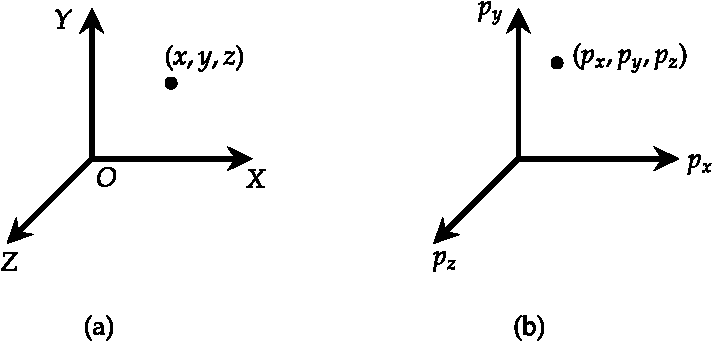
\includegraphics[height=3.5cm,width=8cm]{SP-01}
\end{figure}
\par A space where the three momentum coordinates are represented along the three mutually perpendicular directions is called the momentum space. In Fig. 4.1 (b) the point of a small element in this space $=d p_{x} d p_{y} d p_{z}$\\
\par Fig. 4.1(a) gives only the instantaneous position of a particle anc Fig. (b) gives only the instantaneous momentum. Suppose we want to specify both this position and momentum at a particular instant in a single space. Such a space is called phase space. In phase space a point $P$ has 6 coordinates, $\left(x, y, z, p_{x}, p_{y}\right.$ and $\left.p_{z}\right)$. So it is a 6 dimensional space. Any point $\mathrm{P}$ in this space is called a phase point. The phase point gives a complete description of the dynamical state of the particle at any instant.\\
\par The volume of an infinitesimal element in phase space $=d \tau$
$$
d \tau=d x d y d z d p_{x} d p_{y} d p_{z}
$$
Let us now consider a system consisting of N-particles. For one particle there are 6 coordinates. So for N-particle there are $6 \mathrm{~N}$ coordinates. This means to specify the state of the system completely we need $3 \mathrm{~N}$ position coordinates and $3 \mathrm{~N}$ momentum coordinates. The instantaneous position of a system(i.e., N-particles) can be represented by a single point in the $6 \mathrm{~N}$-dimensional phase space.
\subsection{$\mu$.Space and $\Gamma$-space}
\par The 6-dimensional phase space for a single particle is called the h-space. The $6 \mathrm{~N}$-dimensional phase space for $\mathbf{N}$ particles is termed as -space ( $\gamma$-space). Thus gamma space is built up as the product of $N, \mu$ spaces.\\
\par Suppose a particle has $f$ degrees of freedom. Then to specify its state, f position coordinates and $\mathrm{f}$ momentum coordinates are required.
If there are $N$ particles in this system then to represent the dynamical state of the system at any instant the total number of coordinates required are $N f$ position coordinates and $N f$ momentum coordinates The phase space of the system will be a $2 \mathrm{~N} f$ dimensional space. We can use generalised coordinates to represent a system. Let $q_{i}$ represent the generalised position coordinate and $\mathrm{p}_{\mathrm{j}}$ represent the generalised momentum coordinates. For $N$ independent particles, in the 6 dimensional phase space, there will be $3 \mathrm{~N}$ position coordinates
$q_{1}, q_{2}, \ldots \ldots . q_{N}$ and $3 N$ momentum coordinates $p_{1}, p_{2}, \ldots \ldots \ldots \ldots p_{N}$
\subsection{Phase Cell}
\begin{figure}[H]
	\centering
	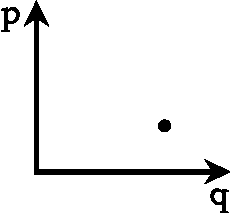
\includegraphics[height=2cm,width=2cm]{SP-02}
\end{figure}
\par Consider a particle in one dimension. Its state can be specified using the position coordinates $p$ and the momentum coordinates $q$ as shown in Fig.4.2 The two coordinates change with time and the representative point moves through phase space and the line traced is called phase line or phase trajectory. Each point on the phase line represents one possible microstate.\\
\textbf{Example}\\
Consider one dimensional harmonic oscillator of mass $m$ and spring constant $\mathrm{k}$. The total energy of the oscillator is $\mathrm{E}=\frac{\mathrm{p}^{2}}{2 \mathrm{~m}}+\frac{1}{2} \mathrm{kq}^{2}$, where $p$ is its momentum and $q$ its position coordinate. If $E$ is constant then this equation represents an ellipse in the phase space.
\begin{figure}[H]
	\centering
	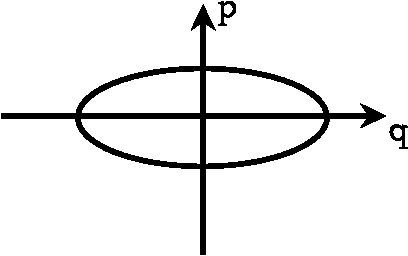
\includegraphics[height=2.5cm,width=4cm]{SP-03}
\end{figure}
$$\frac{q^{2}}{(2 E / k)}+\frac{p^{2}}{2 m E}=1$$
The semi major axis of the ellipse [see Fig. 4.3] is $\sqrt{2 \mathrm{E} / \mathrm{k}}$ and the semi minor axis is $\sqrt{2 \mathrm{mE}}$.\\
\par We can divide the phase space into small volumes called phase cell. In the $\mu$-space of a particle, the volume element $d \tau=d x\  d y \ d z\  p_{x}\  p_y \ p_z$ . $d\tau$  is the volume of a six dimensional cell having sides ${d x, d y, d z}$ $d p_{x}, d p_{y}, d p_{z}$. Such a cell of minimum volume is called a unit cell in the $\mu$-space.
$$(d \tau)_{\min }=\left(d x d y d z d p_{x} d p_{y} d p_{z}\right)_{\min }$$
$$=\left(\delta x \delta p_{x}\right)_{\min }\left(\delta y \delta p_{y}\right)_{\min }\left(\delta z \delta p_{z}\right)_{\min }$$
According to classical mechanics the volume d$\Gamma$
 l can take any minimum value. But in quantum mechanics, according to Heisenberg's uncertainty principle the minimum value of the products is approximately equal to the Planck's constant $h$.\\
$$\text{ So }(d \tau)_{\min }=\mathrm{h} \times \mathrm{h} \times \mathrm{h}=\mathrm{h}^{3}$$
 The minimum value of volume element of $\mu$-space is $h^{3}$, where 3 is the number of degrees of freedom.\\
 \par Consider a system consisting of $\mathrm{N}$ particles having $f$ degrees of freedom each. Then the phase space will be $2 \mathrm{fN}$ dimensional and the volume of the cell be $\mathrm{h}^{\mathrm{Nf}}$.
 \begin{align*}
  \text{The volume}&\text{ of one element in the $\Gamma$ space}\\
  d\Gamma&=\left(\mathrm{dq}_{1} \mathrm{dq}_{2} \mathrm{dq}_{3} \ldots \ldots . d \mathrm{q}_{\mathrm{fN}}\right)\left(\mathrm{dp}_{1} \mathrm{dp}_{2} \mathrm{dp}_{3} \ldots \ldots \mathrm{dp}_{\mathrm{fN}}\right)\\
  \text{The number }&\text{of cells in this volume element is d $\Omega$.}
 \\
 d \Omega&=\frac{\left(d q_{1} d q_{2} \ldots \ldots . d q_{f N}\right)\left(d p_{1} d p_{2} \ldots . d p_{f N}\right)}{h^{N f}}
 \end{align*}
\subsection{ Thermodynamic probability}
 The thermodynamic probability is the number of microstates corresponding to the given macrostate of the system.
 
 As an example consider the distribution of 4 particles in the two halves of a box. There are five macrostates viz., $(4,0),(3,1),(2,2),(1,$, 3) and $(0,4)$ are possible. The thermodynamic probability corresponding to the distribution $(2,2)$ is 6 .\\
 The redistribution or permutation of indistinguishable particles in a cell is meaningless because it does not produce any new microstate and so it is neglected.
 
 Consider the distribution of $\mathrm{n}$ similar particles in $\mathrm{k}$ similar boxes such that $n_{1}, n_{2}, n_{3} \ldots . n_{k}$ particles are in the boxes $1,2,3, \ldots . k$ respectively. Then $n_{1}+n_{2}+n_{3}+\ldots \ldots n_{k}=n$.
 
It can be shown that the number of microstates corresponding to this distribution or its thermodynamic probability $\Omega=\frac{n !}{\pi n_{i} !}$\\
\textbf{Proof}
\begin{align*}
\text{The number of ways of chosing }&n_{1} \text{particles for the first box}\\
&=\frac{n !}{n_{1} !\left(n-n_{1}\right) !}\\
\text{From the remaining particle }&\left(n-n_{1}\right)\text{ we have to chose $n_{2}$ particles }\\
\text{for the box 2. This can be done in }&\frac{\left(n-n_{1}\right) !}{n_{2} !\left(n-n_{1}-n_{2}\right) !}\text{ ways. For the box}\\
\text{$3, \mathrm{n}_{3}$ particles can be chosen in }& \frac{\left(\mathrm{n}-\mathrm{n}_{1}-\mathrm{n}_{2}\right) !}{\mathrm{n}_{3} !\left(\mathrm{n}-\mathrm{n}_{1}-\mathrm{n}_{2}-\mathrm{n}_{3}\right) !}\text{ ways and so}
\intertext{So the total number of meaningful ways of arranging $n_{1}, n_{2}, n_{3} \ldots . n_{1}$ particles in boxes $1,2,3 \ldots . \mathrm n{k}$ respectively is,}
\Omega=\frac{n !}{n_{1} !\left(n-n_{1}\right) !} &\times \frac{\left(n-n_{1}\right) !}{n_{2} !\left(n-n_{1}-n_{2}\right) !} \times \frac{\left(n-n_{1}-n_{2}\right) !}{n_{3} !\left(n-n_{1}-n_{2}-n_{3}\right) !} \times \ldots, k\text{ terms}\\
\Omega&=\frac{n !}{n_{1} ! n_{2} ! n_{3} ! \ldots \ldots n_{k} !}\\
\text{For the }i^{\text {th }}\text{ distribution then the probability}\Omega_{\mathbf{i}}&=\frac{\mathbf{n} !}{\pi \mathbf{n}_{\mathbf{i}} !}
\end{align*}
\subsection{Statistical Ensemble}
A collection of particles is called a system. A number of systems constitute an ensemble. Sometimes it is difficult to study the behaviour of a complex system. But a suitably created ensemble help us to compute the statistical behaviour of the system
\begin{figure}[H]
	\centering
	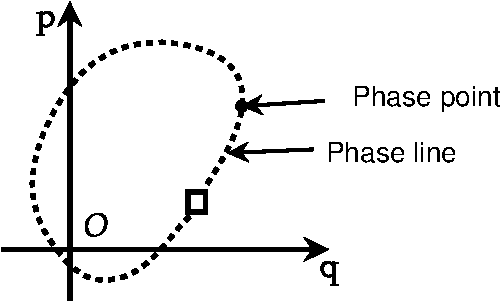
\includegraphics[height=3cm,width=5cm]{SP-04}
\end{figure}
The phase line of a single system is as shown in Fig. 4.4. Each phase point on the phase line emerges from the previous point, with passage of time, in accordance with the laws of mechanics. Suppose we want to compute a physical quantity of the system. Usually what we do is we find its time average over a certain interval of time. But Gibbs reduced this time dependent picture by a static picture. According to this model, the entire phase line shown by dotted line, in Fig.4.4 exists at one time. Then each phase point represents a separate system, with the same macroscopic properties $(N, V, E)$ but a different microscopic state where $\mathrm{N}$ is the total number of particles in the system, $V$ its volume and $E$ its total energy. i.e., we just imagine a large number, (almost infinity) of systems, which are similar in structure to the system under consideration, but placed at random in the accessible, unobservable microscopic states. Now we don't take the time average but take an average over this artificially created group of systems created simultaneously one time. This collection of replicas of similar, independent noninteracting systems is calle an ensemble. Gibbs assumed that the time average of some property of a system in equilibrium is same as the instantaneous ensemble average. This is called the ergodic hypothesis.

All the members of the ensemble which are identical in $\mathrm{N}, \mathrm{V}, \mathrm{E}$ are called elements.
\begin{figure}[H]
	\centering
	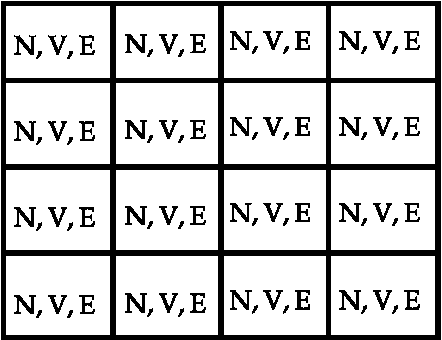
\includegraphics[height=3.3cm,width=4cm]{SP-05}
\end{figure}
In Fig. $4.5 \mathrm{~N}, \mathrm{~V}, \mathrm{E}$ represents one system. A collection of such system constitute an ensemble.
\subsection{Characteristics of an ensemble}
\begin{enumerate}
	\item  The elements of an ensemble are identical in structure. i.e., they have the same macroscopic state.
\item  The elements differ in their miccroscopic state. i.e., they diffet from each other in the position coordinates and momentum coordinates.
\item  The various elements do not interact each other.
\item  Each element of the ensemble behaviour independently obeying the laws of mechanics.
\item  The elements of the ensemble are the mental copies of the system under consideration. But the system is a physical object, whose properties are to be evaluated. The elements help us to use the probability theory.
\end{enumerate}
\subsection{Ensemble average}
The average value found out at a fixed time over all the elements in an ensemble is called an ensemble average. The ensemble average will be equal to the time average when the system contains a large mumber of particles (molecules) and the ensemble contains a large namber systems (both almost infinite in number).
\subsection{Liouville's Theorem}
The condition of an ensemble at any time can be specified by the density $\rho$ with which the phase points are distributed over the phase apace.  It is called the density of distribution and is a function of the position coordinates (q) and momentum coordinates (p).

The dynamical state of a system at any instant of time can be represented by a point in the phase space.  This point will not be stationary, but will move along a certain trajectory. The trajectory is determined by the equatio of motion,
$$\dot{q}_{i}=\frac{\partial \mathrm{H}}{\partial \mathrm{p}_{i}}\text{ and}$$
$$\dot{p}_{i}=-\frac{\partial H}{\partial \dot{q}_{i}}$$
where $H=H\left(q_{i}, p_{i}\right)$ is the Hamiltonian of the system. Due to this motion, the density $\rho$ of the system in phase space changes with time.

Lioville's theorem gives the value of $\frac{\partial \rho}{\partial t}$ at a given point in phase space.
Liouville's theorem states that the density of systems in the neighbourhood of some given system in phase space remains constant in time.
\begin{equation}
\frac{d \rho}{d t}=\frac{\partial \rho}{\partial t}+\sum_{i}\left(\frac{\partial \rho}{\partial q_{i}} \dot{q}_{i}+\frac{\partial \rho}{\partial p_{i}} \dot{p}_{i}\right)=0
\end{equation}
The sum of the two terms give the total change in density with time, Liouville's theorem states that the variation of density with time is zero.i.e., the total rate of change of density $d\rho/d\tau$ near any selected phase point of a system, as it moves through the phase space is zero.

This is known as the principle of the conservation of the density in phase.  This implies that the distribution of phase points move in phase space like an incompressible fluid.\\
\subsection{Different Types of Ensembles}
Depending on the behaviour of the constituents of an ensemble with respect to the surroundings, ensembles are classified into mainly three types (i) Microcanonical ensemble (ii) Canonical ensemble and (iii) Grand canonical ensemble.\\
Uniform ensemble\\
- If the density in phase space is constant it is called uniform ensemble.
\subsection{Microcanonical Ensemble}
Microcanonical ensemble is a collection of independent systems of constant volume separated from the neighbours with rigid impermeable adiabatic walls. $N, V$ and $E$ remains constant, $N$ is the total number of particles in the system. $V$ and $E$ are the volume and energy of the system [See Fig. 4.6] respectively.\\
Consider a system for which the total energy $H(q, p)=E$ is conserved. i.e., $E\left[q_{1} \ldots \ldots . q_{f}, p_{1} \ldots \ldots p_{f}\right]=a$ constant\\
The locus of all the phase points having the same value for the energies in the phase space is called an energy surface or ergodic surface. A number of such energy surfaces can be constructed in the phase space. Each energy surface divides the phase space into two parts, one of lower energy and the other of higher energy. Since the two are of different energies they do not intersect each other.
\begin{figure}[H]
	\centering
	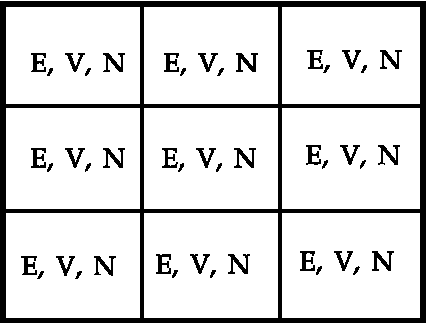
\includegraphics[height=3.3cm,width=4cm]{SP-10}
\end{figure}
Let $\mathrm{E}$ and $\mathrm{E}+\delta \mathrm{E}$ be two neighbouring ergodic surfaces. The phase volume in between the two surfaces encloses a certain number of phase points and will be a constant. Let us assume the density to be zero for all values of energy except in a narrow range of energy between $E$ and $\mathrm{E}+\delta \mathrm{E}$ [See Fig. 4.7]. Then the ensemble specified in terms of $\rho$ as, is called a micro canonical ensemble.

$\rho$ is a function of energy. Here $\rho$ is constant and hence $E$ is also a constant. So the ensemble is in statistical equilibrium. Since $\rho$ is a constant within the energy shell, the distribution of phase points is also uniform, by Lioville's theorem. As the ensemble is in statistical equilibrium, the average properties predicted will not change with time [See Fig. 4.7].\\
\begin{figure}[H]
	\centering
	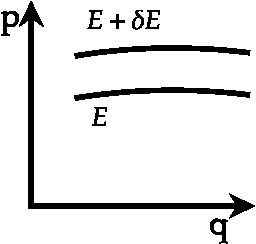
\includegraphics[height=2.5cm,width=2.5cm]{SP-07}
\end{figure}
A microcanonical ensemble can be obtained from a uniform ensemble by neglecting those systems whose phase points do not lie within the phase space corresponding to the energy range between $\mathrm{E}$ and $\mathrm{E}+\delta \mathrm{E}$.

A microcanonical ensemble is an idealised concept and hence cannot exist in practice because the systems which we come across always interact with their surroundings, either thermally or mechanically.
In microcanonical ensemble there is exchange of neither energy nor particles (molecules) among the systems.
Canonical Ensemble\\
Canonical ensemble is a collection of independent systems of constant volume separated from the neighbours by rigid, impermeable, diathermic walls so that the systems are in thermal equilibrium. The particles can exchange energy and hence all the systems will attain the same temperature. The systems have the same temperature $\mathrm{T}$ and constant volume $\mathrm{V}$. The number of particles $\mathrm{N}$ is also a constant. In canonical ensemble systems can exchange energy and not particles. [See Fig. 4.8]
\begin{figure}[H]
	\centering
	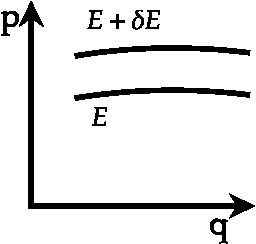
\includegraphics[height=2.5cm,width=2.5cm]{SP-07}
\end{figure}
\subsection{Grand Canonical Ensemble}
\begin{figure}[H]
	\centering
	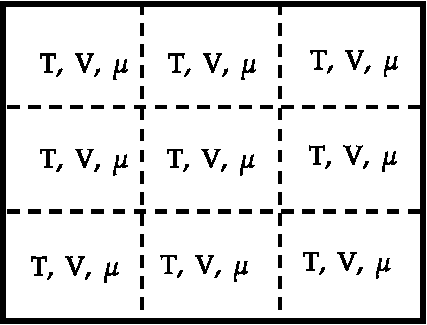
\includegraphics[height=3cm,width=4cm]{SP-09}
\end{figure}
Grand Canonical ensemble is a collection of independent systems of constant volume but open and separated from its neighbours by diathermic permeable membrane so that both material and energy can be exchanged between the neighbours. Since there is exchange of energy, the energy of each system $E$ is not a constant. Also there is exchange of particles, so the total number of particles in each system do not remain constant. The temperature T, volume $\mathrm{V}$ and chemical potential $\mu$ of each system remain constant [See Fig. 4.9].\\
In grand Canonical ensemble there is exchange of both energy and particles (molecules) among the systems.
\subsection{Statistical Equilibrium}
A system of particles which does not interact with any other system so that its total energy remains constant is called an isolated system. A small part of the isolated system which is still macroscopic is called a subsystem. Subsystem interacts with other parts of the system and hence is not isolated.\\
If in any macroscopic subsystem of an isolated system, the average number of particles per unit volume and the average energy per particle are equal to their mean values, then the isolated system is said to be in statistical equilibrium i.e, when the mean values of macroscopic parameters like pmessure, volume, ternperature etc. are independent of time, the systern is in equilibrinarn. If the systern is foumd with equal probability in cach of its possible quantum states then the isolated system is in statistical or thenmodynamic equilibrinm. In tenms of density p, the condition for an ensemble to be in statistical equitibrinm is $\left(\frac{\partial \rho}{\partial t}\right)_{q, p}=0$, i.e, $\rho$ is independent of time at all points in the phase space for the ensemble. For this p must be a function of some property\\
of the ensemble which does not depend on time.
\subsection{Postulate of Equal a priori probability}
Consider an isolated 'many particle system' in equilibrium. We want to know the probability for any one particle to be in a given specified state. The answer to this is given by the a priori postulate.\\
* All accessible microstates corresponding to possible macrostates are equally probablem. This is the most fundamental postulate of statistical mechanics. This means that the probability of finding the particle in any one region is identical with that for any other region of equal volume, under similar conditions.\\
\textbf{Postulates of Statistical Mechanics}
\begin{enumerate}
	\item Any system (say gas taken a cylinder) consists of a large number of particles (atoms, molecules) which are in continuous random motion.
	\item The particles behave like very small elastic spheres.
	\item All the cells in the phase space are of equal size.
	\item All accessible microstates corresponding to possible macrostates are equally probable (equal a priori probability). This postulate means that no microstate is given any preference over the others. Hence the probability of occurrence of a particular macrostate is proportional to the number of microstates corresponding to that given macrostate. Thus the probability that the system will possess energy $E$ is proportional to $\Omega$ (E). i.e. $P E x \Omega(E)$ or $P(E)=C \Omega(E)$ where $\Omega(E)$ is the number of corresponding microstates and $C$ is the constant of proportionality.
	\item  The equilibrium state of a gas corresponds to the macrostate of maximum probability.
	\item  The total number of molecules is a constant. This is in accordance with the law of conservation of matter. Let $n_{1}, n_{2}, n_{3} \ldots \ldots$ be the number of molecules in the cells $1,2,3, \ldots \ldots$ and $N$ be the total number of molecules. Then, $\mathrm{N}=\mathrm{n}_{1}+\mathrm{n}_{2}+\mathrm{n}_{3}+\ldots=\mathrm{a}$ constant.
	\item  The total energy of the system remains constant. This is in accordance with the law of conservation of energy. Let the energy of each particle in the cells $1,2,3, \ldots \ldots \mathrm{k}$ be $E_{1}, E_{2}, E_{3} \ldots \ldots E_{K}$
\end{enumerate}
